\section{Explainability} \label{sec:explainability}
\citet{Doran2018}, carried out a frequency analysis of explanation terms within documents from relevant research communities.
They highlight how different circles have different approaches to the concept of explainability and how, even within the same group, terms are used interchangeably.
In particular, they note the overloading of the notion of \textit{explanation} with that of \textit{interpretability}; a concept that is often defined within the xAI community as necessary for, but distinct from, explainability.
The use of \textit{interpretable}, as signifying the property belonging to a system whose inner workings are accessible, can be found, for example, in the recent paper \citep{gilpin2018explaining}.
In other recent works the two terms are conflated, for example in \citep{mittelstadt2019explaining}, \citep{guidotti2018survey} and in the influential work by \citet{doshi2017towards}.
This seems to prove the point made by \citet{Lipton2016} in the widely-cited paper \enquote{The Mythos of Model Interpretability}, that \enquote{the task of interpretation appears underspecified. Papers provide diverse and sometimes non-overlapping motivations for interpretability and offer myriad notions of what attributes render models interpretable}.

Most works, even those that blend the notions of interpretability and explainability, seem to agree on the end-goal that implementing such a concept should have; that is, to \enquote{summarize the reasons for neural network behavior, gain the trust of users, or produce insights about the causes of their decisions} \citep{gilpin2018explaining} by being able to \enquote{explain or to present in understandable terms to a human} \citep{doshi2017towards}.
Where the consensus diverges, is in defining what constitutes an explanation and in fixing the desiderata that it may have.
\citet{mittelstadt2019explaining} identify two broad classes of interpretability/explainability within the literature: \textit{transparency} (also called \textit{ante-hoc} explainability) and \textit{post-hoc} interpretability.
The former type deals with the internal workings of a system while the latter applies to its external behaviour.
\citet{Lipton2016} identifies three explanations that can make a model transparent: a mechanistic understanding of the workings of the system in its entirety, of the individual components or of the algorithm.
A system may be made post-hoc interpretable by way of natural language explanations, visualisations or interactive interfaces, among others.
These methods often do not precisely clarify the exact working of a model, but \enquote{they may nonetheless confer useful information for practitioners and end-users of machine learning}.
\citet{Biran2017} note how the transparent or \textit{white-box} paradigm was sufficient for classic rule-based models but - with the advent of contemporary machine learning models - is no longer useful.
They argue that it is nowadays unreasonable to expect that any domain expert be able to understand a prediction if they are not also a machine learning specialist.
To address this issue, they propose a \textit{natural language generation system}; that is, a \textit{post-hoc} explanation in the categorisation by \citet{mittelstadt2019explaining}.

A widely-recognised feeling, closely connected with the already identified lack of shared working definitions, seems to be that researchers of explainable AI are ignoring the enormous corpus of existing work in the fields of philosophy, psychology, cognitive and social sciences and human-computer interaction.
This feeling of disconnect is echoed by \citet{gilpin2018explaining} who point out how philosophical texts have long debated what constitutes an explanation and by \citet{mittelstadt2019explaining} who explicitly say how \enquote{many different people, be they lawyers, regulators, machine learning specialists, philosophers, or futurologists, are all prepared to agree on the importance of explainable AI [...] very few stop to check what they are agreeing to, and to find out what explainable AI means to other people involved in the discussion}.
The fact that explainable AI researchers seem to be intent on \enquote{reinventing the wheel} is stated most strongly by \citet{miller2018explanation}, whose paper \enquote{Explanation in Artificial Intelligence: Insights from the Social Sciences} is based on the premiss that \enquote{most of the research and practice in this area seems to use the researchers' intuitions of what constitutes a `good' explanation} and argues for the adoption of the existing research in the social sciences.
The author's views are well summarised by the position xAI is set to occupy in Figure \ref{fig:xai-position}.
The feeling is that explainable AI researchers are calling their methods an \textit{explanation} based on purely personal views and are thus building explanations that only work for themselves; in other words, \enquote{the inmates are running the asylum} \citep{Miller2017}.
The following quote from \citet{guidotti2018survey} seem to perfectly sum up the state of the research in the field: 
\begin{quotation}
	It is evident that the research activity in this field completely ignored the importance of studying a general and standard formalism for defining an explanation, identifying which are the properties that an explanation should guarantee, e.g., soundness, completeness, compactness and comprehensibility. Concerning this last property, there is no work that seriously addresses the problem of quantifying the grade of comprehensibility of an explanation for humans, although it is of fundamental importance. 
	
	\hfill \citep[pag. 37]{guidotti2018survey}
\end{quotation}

\begin{figure}[htbp]
\centerline{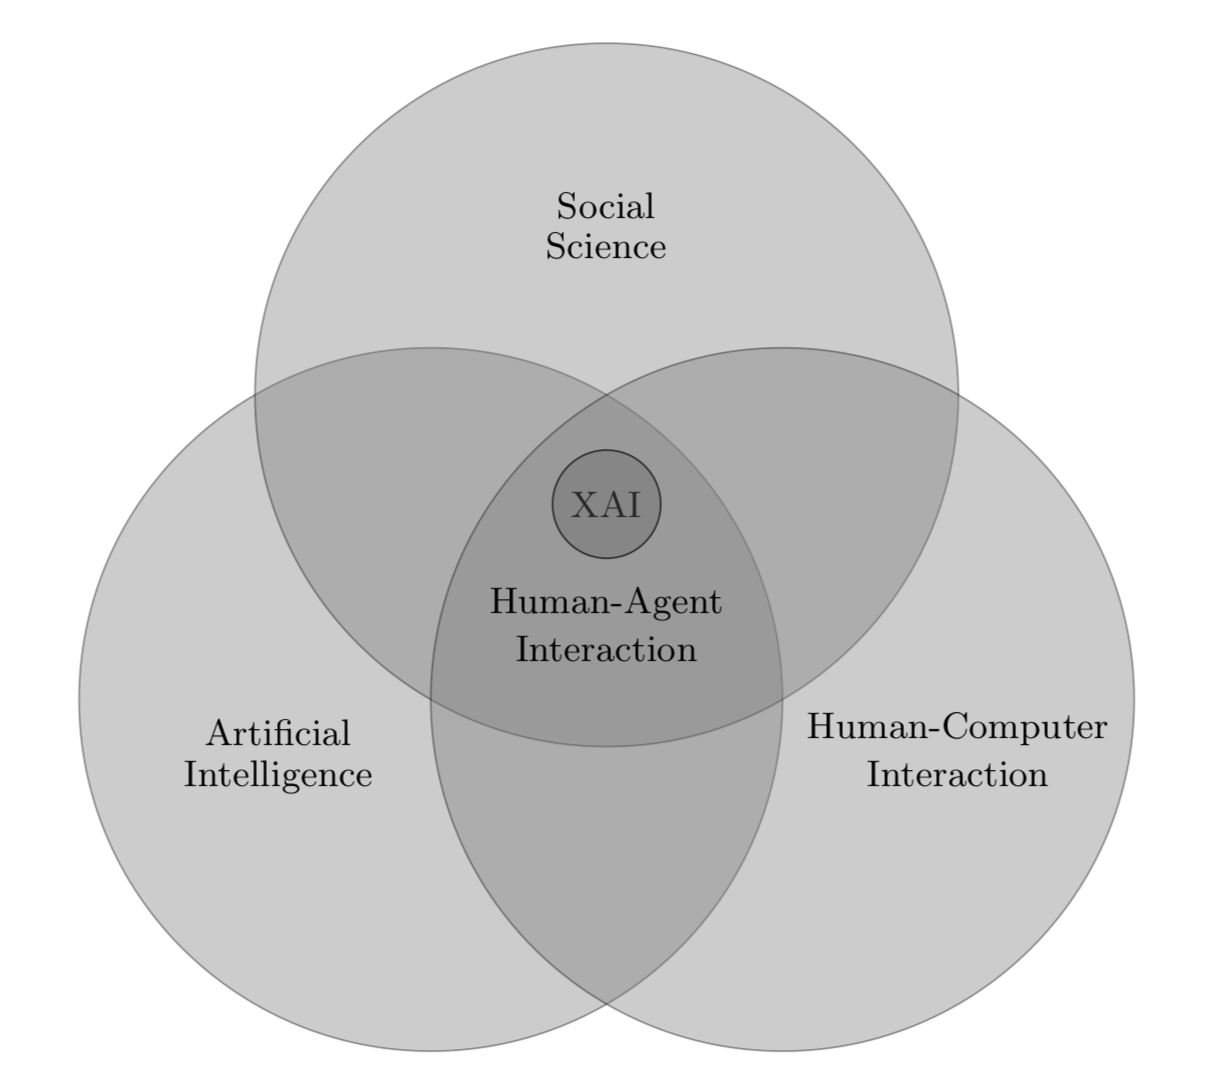
\includegraphics[width=0.5\textwidth]{literature-review/images/xai-position}}
\caption{Venn diagram showing where the field of xAI should \textit{ideally} be positioned \citep{miller2018explanation}.}
\label{fig:xai-position}
\end{figure}

To remedy this state of affairs, there have been a number of works, such as \citep{doshi2017towards}, which have attempted to define what an explanation means and to reach a consensus on it.
The most compelling attempt is in a paper by \citet{Doran2018} (already mentioned in Section \ref{sec:intro-context}) where the authors try to synthesise the current state of affairs into a taxonomy of models:
\begin{itemize}
	\item \textit{Opaque systems}: these are systems that offer no insight into how their internal workings transform the inputs symbols, usually real-world data, into some output, for example labels that classify the data or predictions of unseen cases. 
		All closed-source algorithms fall under this definition.
	\item \textit{Interpretable systems}: this is the vastest category, as the characteristic of these systems is \textit{transparency} i.e., their inner workings are accessible but the onus of comprehensibility falls completely onto the user.  
		The classical example is that of neural networks, where the mapping from inputs to outputs is inspectable by the user who can, theoretically and depending on her skill, interpret them.
		In the case of neural networks this may be a daunting task due to their distributed and non-symbolic nature; in other classes of machine learning models, for example Bayesian networks, the task may be easier as discussed in Section \ref{sec:explainability-in-bayesian-networks}.
	\item \textit{Comprehensible systems}: systems in this category emit additional symbols together with their outputs with the explicit intent of giving the user the means to interpret and understand the automated decisions.
		The additional symbols may be visualisations, natural language text or any other means of demystifying the output.  
		These extra symbols would need to be graded based on the user's expertise, as comprehension is a property that involves both man and machine.
		An example of such a system would be an image classifier that, together with its output, highlighted the parts of the image it used to make its decision.
	\item \textit{Explainable systems}: the highest level in the taxonomy includes those models that emit an explicit \textit{explanation} i.e., a human-understandable line of reasoning.
\end{itemize}
It is recognised that comprehensibility depends not only on the system's characteristics, but also on the user's ability and knowledge, thus implicitly accepting the view that xAI should include elements from the social sciences.
\textit{Comprehensibility} and \textit{interpretability} are considered separate concepts as comprehension requires transparency but interpretation does not, given that the user may reason only over the emitted extra symbols.
This notion of comprehensibility is expanded into that of \textit{real} explainability, based on a notion of \enquote{ability to formulate, for the user, a line of reasoning that explains the decision making process of a model using human-understandable features of the input data} \citep{Doran2018}.

\section{Importance of Explainability} \label{sec:importance-of-explainability}
As noted by \citet{edwards2018enslaving}, \enquote{businesses and governments are increasingly deploying machine learning (ML) systems to make and support decisions that have a crucial impact on everyday life} so, as \citet{gilpin2018explaining} say, \enquote{it becomes necessary for these mechanisms to explain themselves}.
This feeling of urgency and purpose is echoed throughout the reviewed literature; it seems that even if researchers and the field as a whole cannot agree on a definition of explainability (as discussed in Section \ref{sec:explainability}), there is a keen awareness of the need for models to be explainable.
This intense urge to define explainability and, at the same time, to try and create models exhibiting this property, may be counterproductive as the field risks fragmenting into a series of diverging strands, as noted by \citet{abdul2018trends} and visualised in Figure \ref{fig:xai-citation-network}.

\begin{figure}[htbp]
\centerline{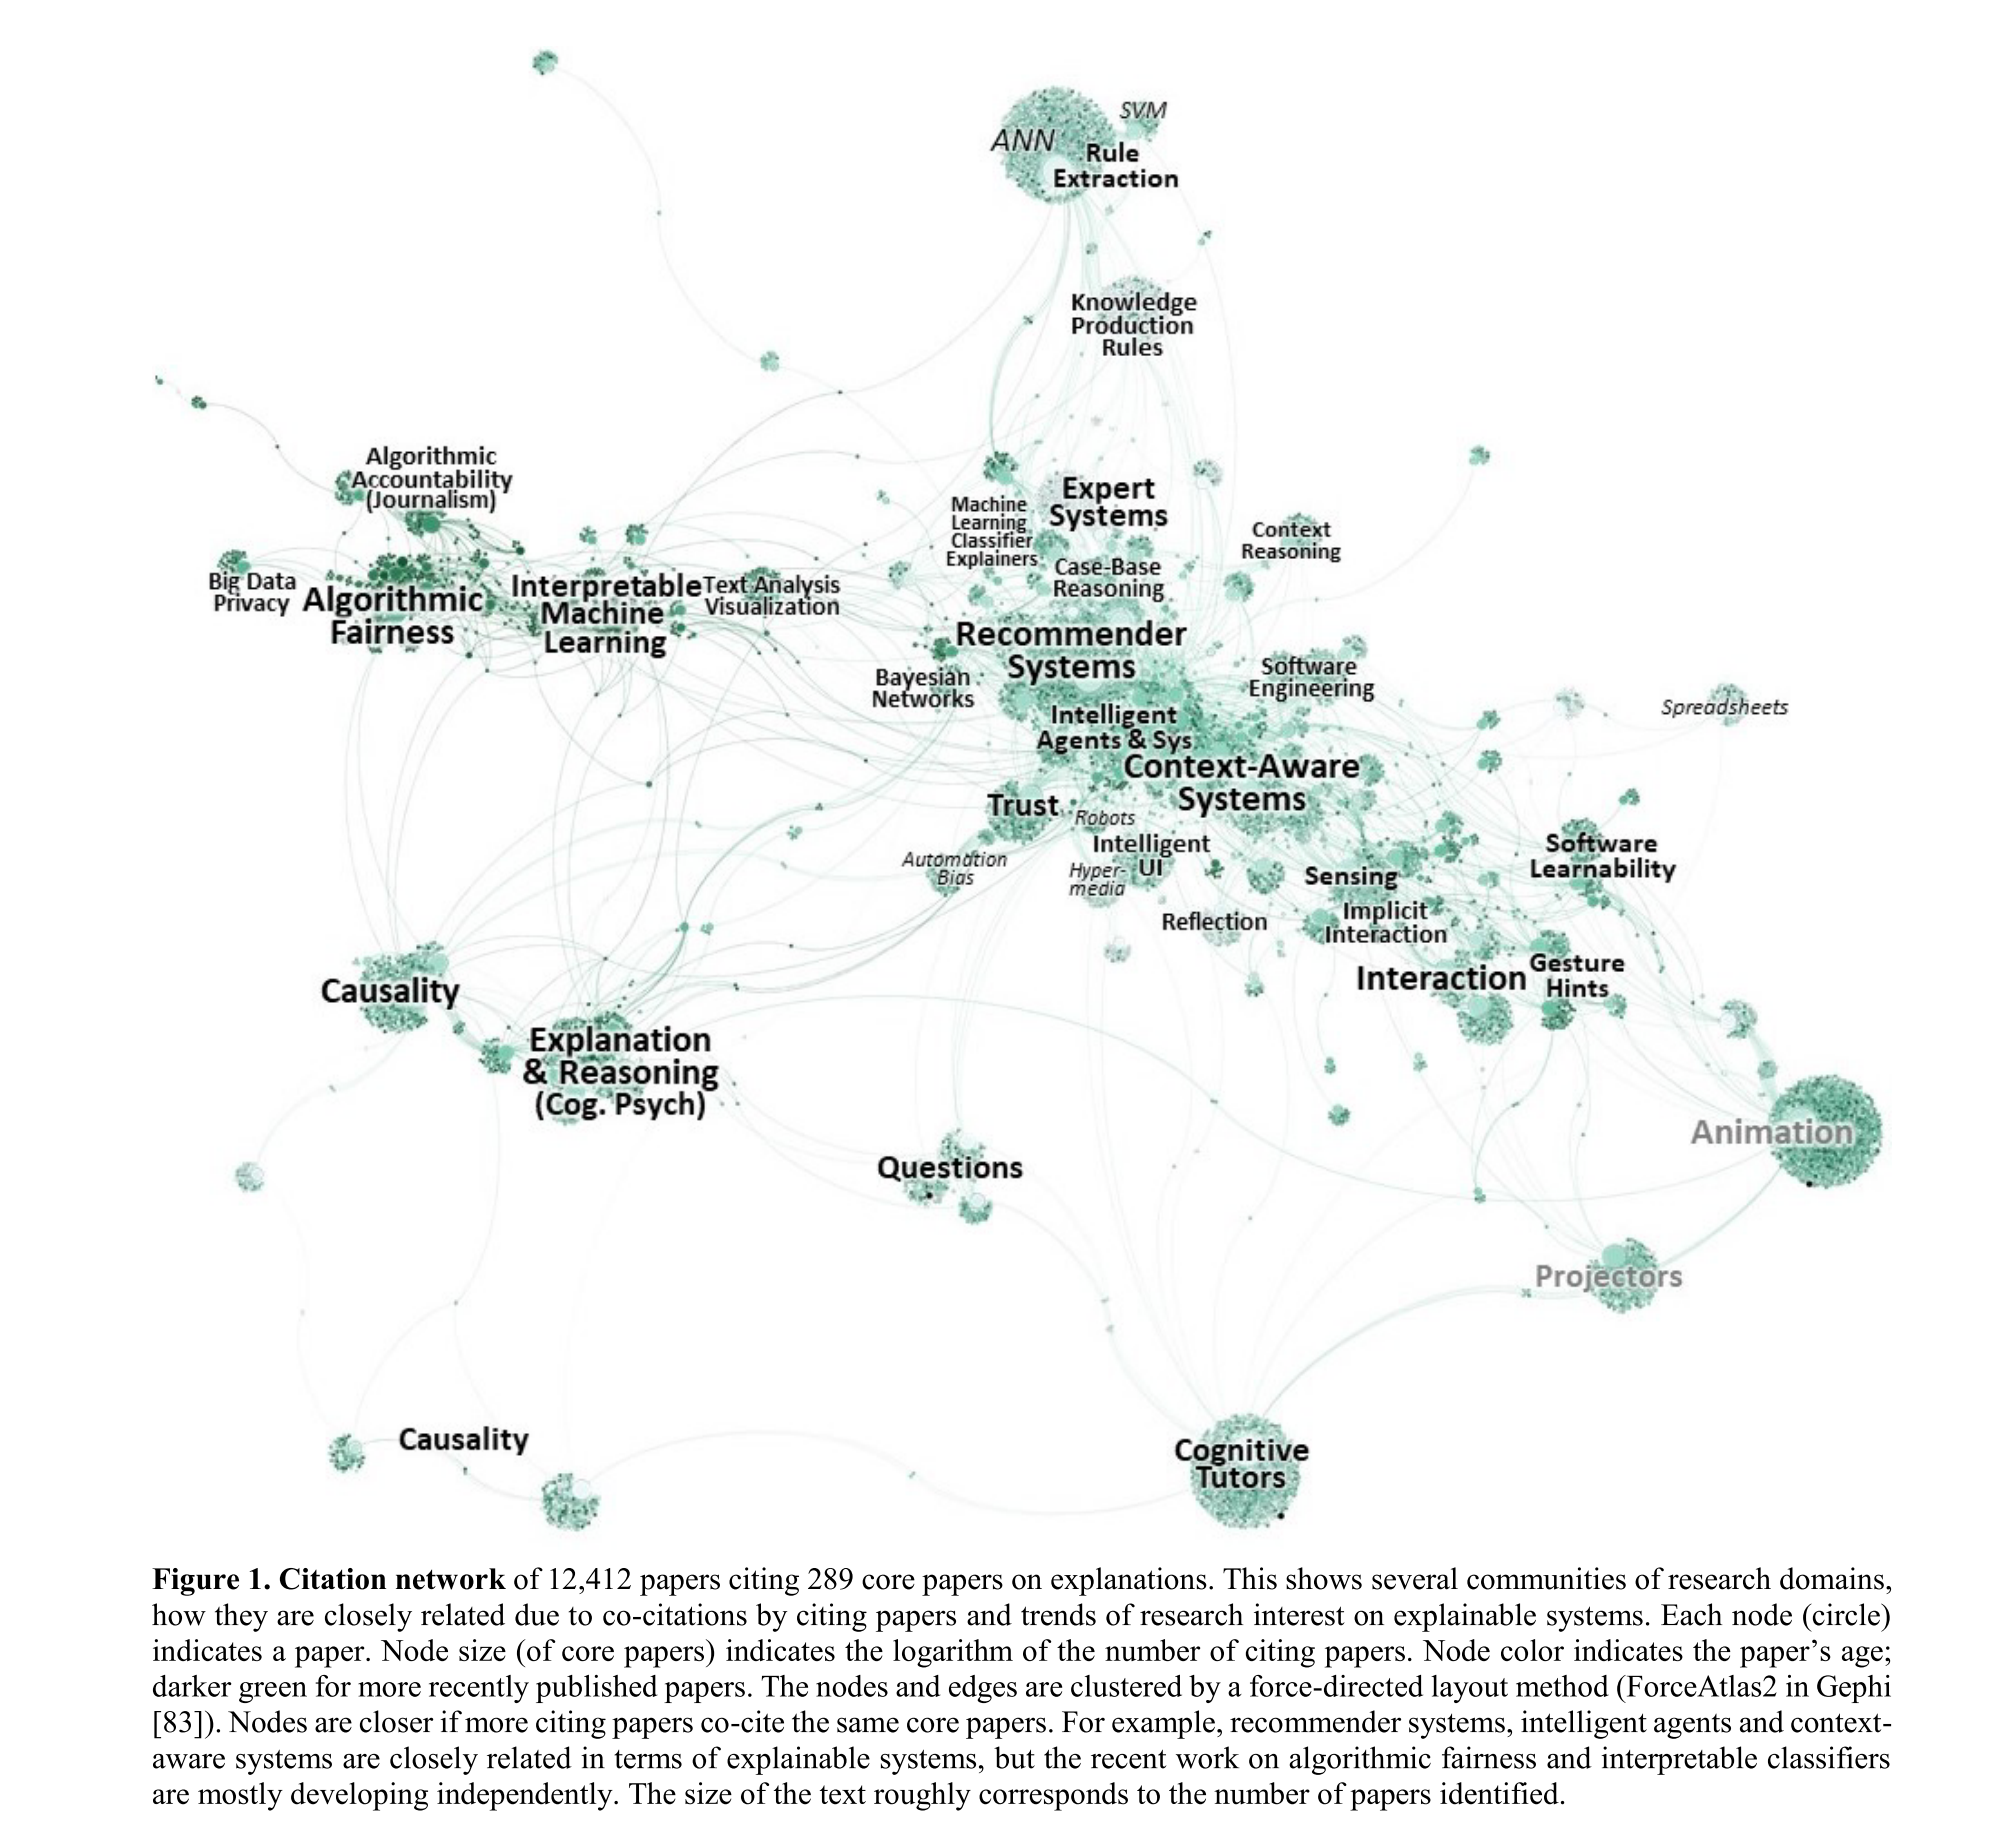
\includegraphics[width=0.8\textwidth]{literature-review/images/xai-citation-network}}
\caption{Citation network that is emblematic in showing the breadth of research strands in the field of xAI \citep{abdul2018trends}.}
\label{fig:xai-citation-network}
\end{figure}

There are a myriad of reasons brought forth as a justification for the development of explainable AI, and we will review these in the following paragraphs, but it seems timely to start with one in particular: the need introduced by the European Union's broad General Data Protection Regulation (GDPR).
The GDPR was approved by the European Parliament in 2016 and came into effect in 2018.
More than one author cites an urgency to conform to this regulation (for example \citet{doshi2017towards}, \citet{gilpin2018explaining}), most likely referring to Article 22 of the regulation that, supposedly, mandates for a \enquote{right to an explanation} from algorithms.
While algorithmic explainability is undoubtedly a commendable objective, it may be the case that this particular reason to strive for it be a false one.
\citet{edwards2018enslaving} posit that Article 22 of the GDPR actually does not contain the publicised right to an explanation but is \enquote{merely a right to stop processing unless a human is introduced to review the decision on challenge} and as the authors point out, there are, nowadays at least, very few systems without a human in the loop.
Secondly, there is no mandate for the \enquote{explanation} to be understandable by humans, so the result obtained might actually be no explanation at all.
If the analysis of \citet{edwards2018enslaving} were correct, then the urgency advocated by many researchers on the grounds of having to conform to the GDPR would, in reality, turn out to be based on no valid reason.

A second motive brought forward for the need for explainability, for example by \citet{gilpin2018explaining} and \citet{abdul2018trends}, is that comprehensible models are much more likely, or even necessary, to engender users' trust.
While this may very probably be the case, no motives are given for why this should be the purpose of explainable AI and not just a desirable by-product of obtaining explainability. 
A reasoning for why trust may stem from explainability can be found in \citep{Kyrimi2016} where it is claimed that \enquote{the lack of trust may be due to the difficulty of understanding how a prediction is inferred from the given data. As Aristotle wrote `we do not have knowledge of a thing until we have grasped its why, that is to say, its explanation'. Hence, explaining a model's reasoning - its inference - could increase trustworthiness.} 
What could be assumed, is that \textit{trust is a prerequisite for explainability} because if the human does not believe the outputs of the machine, there is little hope for an explanation to come into being.

Other authors, for example, \citet{doshi2017towards} and \citet{guidotti2018survey}, frame the issue as one of moral necessity.
One need not look far to find examples of ML models displaying \textit{covert bias} or making decisions we would regard as unethical; a more in-depth investigation would reveal that this was the case even before the popularisation of \enquote{black box} models as are deep neural networks.
\citet{guidotti2018survey} give a reasonably comprehensive list of classic cases that show the risks inherent in not having comprehensible AI.
The oldest of these dates back to the 1970s and 1980s and tells of a system used to screen job applicants that was still seen to discriminate against minorities, even though programmed to ignore people's ethnicity.
In the same vein but much more recently, the American Military discovered that their computer vision system, developed to differentiate between enemy and friendly tanks automatically, had poor accuracy because it had learned to use the background information of the test set photos instead of the pixels representing the actual vehicles.
Both these cases exemplify how an algorithm may make \enquote{wrong} inferences based on spurious or latent information that was already in the data set but that no human could have imagined being relevant.
Other failures epitomise how a model may learn our own social prejudices; for example, a recent Princeton study \citep{caliskan2017semantics} proved how models trained on web text corpora showed marked bias (towards race, gender ...) that reflected the ones present in our own society.
Based on their findings, the authors went so far as to suggest that transparency would not be enough to uproot bias, since the very \textit{semantics} of language reflects prejudice latent in our culture. 

The driving motivation and sense of urgency present in all of the reviewed literature is quite certainly tied to the renewed interest and applicability of AI.
\citet{Preece2018} claims that the interest for explainability is naturally linked to that in AI; if this were true, then it would confirm that a need for transparency is implicit in the field itself.
This would validate the assertion made by \citet{doshi2017towards}, that the need for an explanation stems from an \textit{incompleteness in the formalisation}.
What is meant by this is that optimising for certain objectives may introduce an \textit{unquantifiable bias} into the system, which is very different from mere \textit{uncertainty}.
Mere uncertainty can be rigorously quantified, formalised and reasoned upon by using probability theory; unquantifiable bias is the result of an \textit{incompleteness in formalisation} of the problem that the ML system is tasked with.
For example, this is the case when a system is coded to pursue soft objectives such as \textit{ethics} as such an end-goal may be too abstract and nebulous to be completely formalised.
It might also be the case that a particular objective is far too complex for all its possible outcomes to be exhaustively enumerated.
A good characterisation of objectives leading to incompleteness could be given by applying the concept of \textit{wicked problem} introduced by \citet{Rittel1973} when analysing the issues arising in social planning.
The first defining characteristic of a wicked problem is that the mere definition of the problem in hand is the wicked problem itself, since even its description is dependent on one's idea for solving it; there is no definite locus that one can point to as the source of the problem. 
Other defining features are the absence of \textit{stopping and objective evaluation criteria} and the fact that each solution to a wicked problem is essentially \enquote{one-shot} and unique.  
Even the set of possible solutions and causes are not predetermined and non-stationary. 
The authors noticed how these problems presented a series of defining characteristics, that they were able to generalise into the notion of \textit{wicked problem}.
A classic example are the issues that arise when trying to solve a social planning problem: various parties will have competing objectives and different ideas to obtain them, so no unique best solution is possible; problems are \enquote{at best, only re-solved} \citep{Rittel1973}. 
These situations generally tend to arise when dealing with human values, as there is always a degree of ethical relativism that makes it difficult to develop and evaluate solutions.  
\citet{Lipton2016} is also aware of this and states that \enquote{the demand for interpretability arises when there is a mismatch between the formal objectives of supervised learning and the real world costs in a deployment setting}.
In the presence of such unquantifiable uncertainty, unavoidable in many of the important applications of AI, requiring the resulting model to be open to inspection would make the \enquote{gaps in problem formalization visible to us} and thus enable us to apply our best human judgement to evaluate them and their consequences \citep{doshi2017towards}.
No wicked problem has a solution that is either true or false, but only good or bad; necessarily, the only judge for this can be a human.

\section{Evaluation of Explainability} \label{sec:evaluation-of-explainability}
As concluded in Section \ref{sec:importance-of-explainability}, the fact that ML models operate on incomplete assumptions makes it a necessity to have some form of evaluation of their performance.
As \citet{Lipton2016} states, \enquote{it turns out that many situations arise when our real world objectives are difficult to encode as simple real-valued functions} and this could lead to evident difficulties in optimisation with respect to soft concepts such as ethics and legality which are, however, of paramount importance.
Being able to evaluate an automated explanation lets us \enquote{serve those objectives that we deem necessary but struggle to model formally}.

Unfortunately, the finding outlined in Section \ref{sec:explainability} of there being no consensus on the definition of explainability also necessarily entails that there is no agreed-upon methodology to evaluate such a property.
\citet{doshi2017towards} note as much when they comment \enquote{unfortunately, there is little consensus on what interpretability in machine learning is and how to evaluate it for benchmarking}.
This makes perfect sense because trying to evaluate something without first having defined it, is worse than trying to hit a moving target.
Once again, the feeling shared among many authors is that \enquote{inmates are running the asylum}.

Some authors have tried to put some order in the barrage of proposed methods with \citet{doshi2017towards} providing one of the most compelling attempts.
These authors set out to outline a taxonomy, having noted a \enquote{lack of rigour} and how current interpretability approaches usually fall into two categories: \textit{interpretability in the context of an application and interpretability via a quantifiable proxy}.
 The former approach assumes that \enquote{if the system is useful in either a practical application or a simplified version of it, then it must be somehow interpretable}; the latter sees researchers claim that a model class is interpretable and then present algorithms to optimise within that class.
 In their words, both classes rely on a notion of \enquote{you'll know it when you see it}.
 The taxonomy the authors propose is laid out in Figure \ref{fig:xai-taxonomy} and borrows from methods already standard in human-computer interaction and visualisation; the guiding ideal is that \enquote{evaluation of applied work should demonstrate success in the application} and thus the best kind of evaluation is the one that involves humans the most:
 \begin{itemize}
  \item \textit{Functionally-grounded Evaluations}: at the lowest level of their taxonomy are those methods requiring no human-in-the-loop and that evaluate the quality of an explanation given by a system by using some proxy measure; the advantage is the low cost, but the tradeoff is a lack of specificity.
 A proxy measure that has already been human-validated as regards its explainability, for example a decision tree, a set of rules or a linear model \citep{guidotti2018survey}, may be substitute to estimate the explainability of more complex systems.
 \item \textit{Human-grounded Evaluation}: the second level of evaluation involves humans, albeit not domain expert ones, carrying out simplified versions of the target application; this kind of setup enables the testing of more general notions of explainability.
 \item \textit{Application-grounded evaluation}: this is considered the gold standard evaluation; the authors claim that there is no better way to evaluate explainability that having a domain expert test it in the context of a real task.
In their words, \enquote{the best way to show that the model works is to evaluate it with respect to the task}: \enquote{for example, a visualization for correcting segmentations from microscopy data would be evaluated via user studies on segmentation on the target image task; a homework-hint system is evaluated on whether the student achieves better post-test performance.  Specifically, we evaluate the quality of an explanation in the context of its end-task, such as whether it results in better identification of errors, new facts, or less discrimination}.
\end{itemize}
  
\begin{figure}[htbp]
\centerline{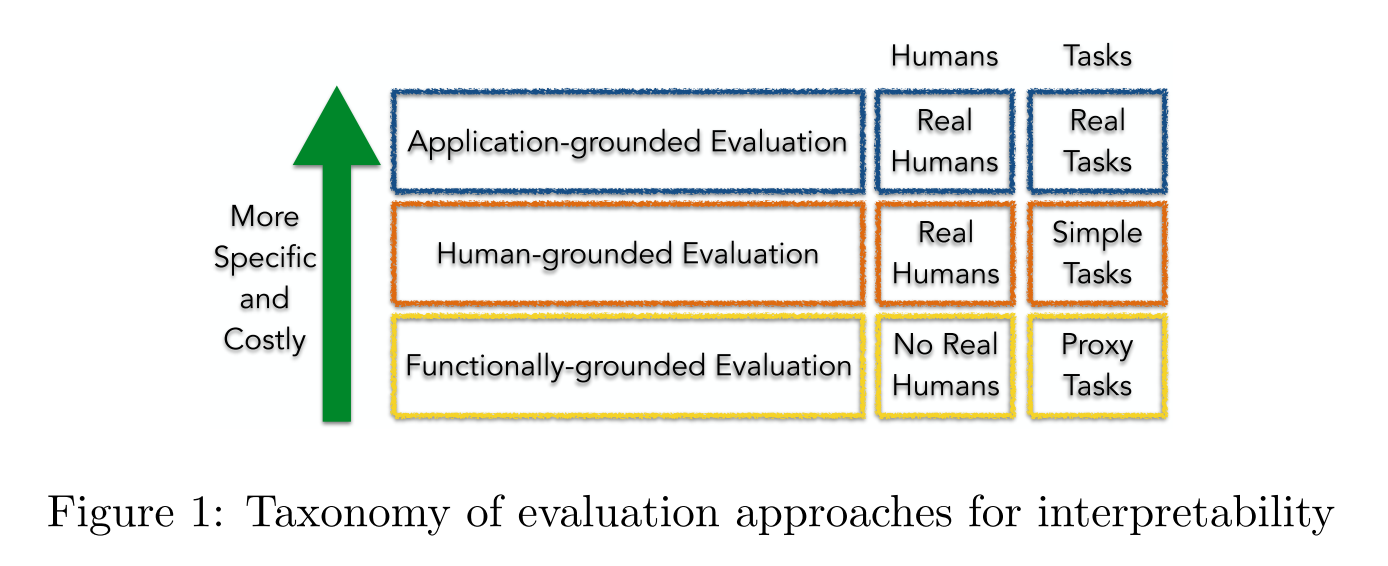
\includegraphics[width=\textwidth]{literature-review/images/xai-taxonomy}}
\caption{Taxonomy of methods for the evaluation of explanations \citep{doshi2017towards}.}
\label{fig:xai-taxonomy}
\end{figure}

\citet{guidotti2018survey} outline a taxonomy developed along a different axis; specifically they identify: 
\begin{itemize}
  \item \textit{methods to explain black box models};
  \item \textit{methods to explain black box outcomes};
  \item \textit{methods to inspect black boxes and methods to design transparent boxes}.
\end{itemize}
An essential factor that the authors identify is that \textit{evaluation is a graded notion}; as also noted by \citet{gilpin2018explaining}: different users, with different expertise and background, may rate the quality of the same explanations very differently.
Another point they make - which is quite novel - is that \textit{time should also be part of an evaluation}: depending on time available a user may prefer a more straightforward or more elaborate explanation.
They end by noting that \textit{very few studies take user expertise and the time taken to understand the proposed explanation into account}.
The concept of \textit{time to understand an explanation} will be part of the methods of this thesis.

The neglect of the human side of explanations is also lamented by \citet{abdul2018trends} who see researchers focusing on creating \textit{mathematically explainable models} at the expense of ones that are usable and practical in real-world situations.
Again, the underlying issue seems to be that xAI researchers are either unaware or are ignoring the sizeable corpus of research available in cognitive psychology, human-computer interfaces and philosophy.
The authors see the opportunity for HCI to bridge the gap between models and users by way of an interactive approach, as opposed to the mainstream static explanations being proposed in the literature.
An interactive explanation may take the form of a dialogue or of various visualisation techniques; the defining characteristic of such an evaluation modality is that it lets the user freely explore the system's behaviour.
\citet{guidotti2018survey}, while discussing the types of data used in ML models, lend credence to the adequacy of this output modality via the statement that \enquote{other forms of data which are very common in daily human life are images and texts. They are perhaps for the human brain even more easily understandable than tables}.

\citet{guidotti2018survey}, though, take the view that evaluation of model \textit{comprehensibility} should be equated to its \textit{complexity}, which is not an opinion that often appears in the reviewed literature.
Basically, the authors are advocating for the use of complexity - the number of identifiable elements in a particular class of model, for example the number of weights in a neural network or of rules in an expert system - as a proxy measure for explainability, if we are framing the issue using the taxonomy proposed by \citet{doshi2017towards} (see Figure \ref{fig:xai-taxonomy}).
This may very well be a valid approach, but there is no supporting evidence for it in the paper itself.

A useful reference for how to set up an experiment falling into the class of either \textit{human-grounded or application-grounded evaluation}, can be found in \citet{stumpf2009interacting}.
In this work the authors set up \enquote{three experiments to understand the potential for rich interactions between users and machine learning systems}; the first, and most relevant, was a \textit{think-aloud study} that investigated \enquote{how machine learning systems should explain themselves to end users, and what kinds of improvement feedback end users might give to the machine learning systems}.
These studies are interesting as a blueprint for future human-centred evaluations, of the type whose absence is being lamented by many authors.

\citet{mittelstadt2019explaining} summarise the existing critiques to offer a clear and direct evaluation of the field of explainable AI as a whole, when they state that:
\begin{quotation}
	no matter the approach taken in xAI, reflexivity \textit{[taking account of itself or of the effect of the personality or presence of the researcher on what is being investigated, clarification not by authors]} is needed to ensure the community actually works towards its normative and practical goals to render models holistically transparent or provide high-quality post-hoc interpretations of model behaviour. Critical questions must be repeatedly asked and answered. For example, will the methods developed make machine learning models more interpretable? More trustworthy to users? More accountable? And to whom will explanations be accessible, comprehensible, and useful? Answering such questions requires considering the methods developed in xAI in the context of prior work in fields addressing such normative and social questions. Local and approximation models may in fact resemble existing, well-known approaches to explanations in the `explanation sciences', which would provide insight.
	
	\hfill \citet[pag. 3]{mittelstadt2019explaining}
\end{quotation}

They then conclude by stating that \enquote{xAI generally avoids the challenges of testing and validating approximation models, or fully characterising their domain}.
From the review of the current state-of-the-art carried out in this section and Sections \ref{sec:explainability} and \ref{sec:importance-of-explainability}, these could both be seen as entirely valid criticisms.
It really seems that the field of xAI as a whole should try and reposition itself as suggested in Figure \ref{fig:xai-position} and not attempt to build methods from first principles, many of which may be outside the domain of expertise of the researchers proposing them.

\section{Explainability in Bayesian networks} \label{sec:explainability-in-bayesian-networks}
Bayesian networks are a popular class of probabilistic models which has enjoyed widespread appeal as a machine learning method, especially in the field of medicine.
The classic \enquote{Asia} toy example of a BN is shown in Figure \ref{fig:asia-bn}; this simple BN is composed of eight nodes, arranged in a parent $\rightarrow$ child relationship; the visualisation makes clear how each one is associated with a \textit{probability distribution}, whose values only depend on the parent nodes (Definition \ref{def:mass-function}).
The popularity of BNs in the area of medicine may be because the formalism (see Section \ref{sec:bayesiannetworks}) \enquote{offers a natural way to represent the uncertainties involved in medicine when dealing with diagnosis, treatment selection, planning, and prediction of prognosis. 
This is due to the fact that the influences and probabilistic interactions among variables can be described readily in a BN} \citep{Lucas2001}; that is, even if the BN model is \textit{complete}, in the sense that every possible probabilistic statement can be computed in it, it is also easy to combine multiple variables of interest into composite statements.
Thus, unlike other popular ML algorithms which may have higher learning performance, BNs enable \textit{reasoning} on the model (for example by using the algorithms presented in Subsection \ref{subsec:bnupdating}).
Another attractive feature of BNs is their relatedness to the class of \textit{causal networks}, popularised by the groundbreaking work of \citet{Pearl1988}; for all intents and purposes, a causal network is simply a Bayesian network where all the relationships represent a causal effect.
Nonetheless, \textit{BNs are not considered as inherently interpretable by the literature}, and thus, a series of methods were developed to address this shortcoming.
\citet{timmer2015explaining} note this in the introduction to their paper by stating that \enquote{for non-statistical experts, however, Bayesian networks may be hard to interpret. Especially since the inner workings of Bayesian networks are complicated they may appear as black box models}, \enquote{the interpretation of BNs is a difficult task, especially for domain experts who are not trained in probabilistic reasoning}.

\begin{figure}[htbp]
\centerline{\includegraphics[width=0.8\textwidth]{literature-review/images/asia-bn}}
\caption{Classic example of Bayesian network [\href{https://www.norsys.com/WebHelp/NETICA/X_Example_Bayes_Net.htm}{Norsys Software Corp.}].}
\label{fig:asia-bn}
\end{figure}

The best overview of the state of explainability of BNs, that will also be used as a framework for the methods developed in this thesis, is given by \citet{lacave2002review} in the paper \enquote{A Review of Explanation Methods for Bayesian Networks}; here the authors identify various classification criteria for an explanation given by a BN:
\begin{itemize}
  \item \textit{description} vs. \textit{comprehension}: the former consists in displaying the data set or providing further details regarding the output, the latter attempts to guide the user in understanding the model's conclusions.
  \item \textit{micro-level} vs. \textit{macro-level}: detailed description of how a single node in the network is affected vs. showing the main lines of reasoning.
  \item \textit{linguistic} vs. \textit{graphical}: \enquote{the most direct and intuitive way of showing the information embodied in a Bayesian network is to display the corresponding graph}.
  When presenting probabilities, \citet{henrion1990qualtitative} strongly suggest that these be \enquote{linguistic probabilities} i.e., for the quantitative probabilities inherent in the model to be converted to a qualitative equivalent.
  This is validated by research showing that linguistic expressions of probability are better understood than the equivalent numerical representation. 
  Some of the many models surveyed in the paper use colours, shading and line thickness to represent the salience of links and nodes.
  The work carried out in this thesis will extensively use both linguistic and graphical explanations; the probabilities will also always be linguistic.
\end{itemize}
When compared with the taxonomies already presented in Section \ref{sec:explainability}, it is obvious that these methods applied to a BN, would make it a \textit{comprehensible system} or \textit{post-hoc explainable} because the model would be emitting extra symbols (graphical, linguistic ...) geared towards explaining its outputs.

The authors also identify the three components of BNs that need to be explained: the \textit{evidence}, the \textit{model} and the \textit{reasoning}.
The first of these \enquote{consists of determining which values of the unobserved variables justify the available evidence} and is, in general, done by finding the solution to the most probable explanation problem (Definition \ref{def:mpe}).
The explanation of the model is considered a \textit{static} explanation (as opposed to \textit{dynamic} ones, shortly be covered) and is simply the process of linguistically or graphically displaying the information already present in the data.
The final element which needs explaining is what would most commonly be called an explanation in xAI circles, is the reasoning behind the model's outputs; a system may accomplish this by providing a justification for its outputs, for the results it did not give or via hypothetical reasoning.
The last of these is maybe the most important, because it is paramount for any system, not just a BN, to be able to explain the reasons behind its outputs; returning to the medical setting, it was seen that physicians, in particular, are very reluctant to accept the advice of a machine if they cannot understand how it was obtained.
A BN, unlike other ML systems, can also innately exhibit evidence for why it did not provide the output expected by the user and can also reason \textit{counterfactually} i.e., provide alternative lines of reasoning.
This will also be an important part of the work carried out in this thesis, as \enquote{counterfactuals}/\enquote{what-if analysis} will be used to help medical experts extract knowledge from data. 
These last two capabilities of Bayesian networks are particularly important, from an explainability perspective, in the light of the findings by \citet{miller2018explanation} regarding the nature of explanations from a psychological perspective.
The conclusions are that \textit{explanations possess four primary characteristics}:
\begin{itemize}
  \item Explanations are \textit{contrastive}: that is people do not ask why an event happened but why another event did not happen instead.  
  A Bayesian network, as noted in the previous paragraph, is capable of modelling counterfactuals which enables it to naturally give contrastive reasonings.
  \item Explanations are \textit{selected}: people expect the explanation given to them to have been selected based on some criterion or cognitive bias; they do not expect a complete recount of all causes of an event.
  A BN has the ability to flexibly combine its constituent variables into an output and thus its explanations can be selected based on some criteria or be \textit{partial}, for added simplicity; a BN's outputs needn't be \textit{complete} i.e., constituted of all its parameters, unlike those of non-local models (for example, neural networks).
  \item To people, probabilities are not as important and not as well understood as \textit{causal} relationships.
  BNs, as already mentioned, are closely related to \textit{graphical causal models}, so their explanations have the possibility of being based on causal grounds. \citep{Lipton2016}, \citet{rani2006empirical}
  \item Explanations are \textit{social}: that is they involve an \textit{explainer} and an \textit{explainee}.  
  This is recognised in \enquote{Conversational Processes and Causal Explanation} by \citet{Hilton1990}, the most important work on the social aspects of conversation, who supports the view that every \textit{explanation} is a \textit{conversation}. 
  A dialogue is an example of a \textit{dynamical explanation}, in the framework set out by \citet{lacave2002review}; these authors also recognise that an explanation \enquote{always means explaining something to somebody} and thus that \enquote{one of the key features of an effective explanation is the ability to address each user's specific needs and expectations, which primarily depends on the knowledge he/she has}.
  	  So \enquote{In the case of a Bayesian network, the explanation generated for a user that is familiar with the concepts of prevalence, prior/posterior odds and likelihood ratios should be very different from the explanation generated for a user who has never heard about them}.
  	  \citet{lacave2002review} again recognise that explainability is a graded notion but go further to note that practically all explainable BN systems have made the assumption of a \textit{fixed user model} thus ignoring the possibility of users having varying levels of knowledge.
  	  However, some of the systems surveyed in the review make a step in that direction by incorporating an \textit{importance threshold} mechanism that would let the user only display certain items; this enables these systems to display varying levels of detail without having defined a particular user model.
\end{itemize}
A \textit{dialogical} explanation could probably make a BN an example of \textit{explainable system}, in the framework developed by \citet{Doran2018} and \textit{post-hoc explainable system} in that of \citet{mittelstadt2019explaining}.

Bayesian networks, without any additional explainability methods, would most probably fall into the class of \textit{interpretable systems}, as do many other ML models, in the taxonomy set forth by \citet{Doran2018}.
Though, based on this review of the literature, it could be justifiably suggested that Bayesian networks are better equipped than other machine learning models to provide a meaningful explanation to humans.
This could be claimed because it is quite widely believed that our brains, and thus our psychology, are near-optimal problem-solvers and as such approximate optimal Bayesian solutions.
A standard view in the fields of psychology and neuroscience, as noted by \citet{Bowers2012}, is that our brain processes approximate the \textit{rational player} as presented in the Dutch Book Argument (see Ch.7 of \citet{anand2009handbook}) and are thus Bayesian in nature.
It is also worth noting that this view has recently been challenged, for example by \citet{Bowers2012}.
This said, even if our brains were not inherently Bayesian, the characteristics of Bayesian networks make them more capable than other ML models in being able to generate explanations tailored to our cognitive biases and psychology, as discussed when presenting the characteristics of an explanation as identified by \citet{miller2018explanation}.